\subsubsection{简介}
近年来，NISQ 设备取得了显著发展。为了应对模拟大规模量子线路这一具有挑战性的任务，经典计算机上的各类模拟器也迅速发展。目前，量子线路模拟器可分为两大类：
\begin{itemize}
    \item 状态向量模拟：状态向量方法直接模拟量子态演化。在 \MindQuantum\ 中，\code{"mqvector"} 属于这一类别。不过，该方法需要存储完整状态信息，因此内存需求会呈指数增长。
    \item 张量网络模拟：张量方法通过收缩张量网络完成模拟 \cite{Huggins_2019,PhysRevLett.128.030501}。
\end{itemize}

在张量网络方法中，量子线路被表示为一个张量网络：单量子比特门用二阶张量描述，双量子比特门用四阶张量描述，$n$ 量子比特门则用 $2n$ 阶张量描述。因此，模拟量子线路就转化为收缩相应张量网络的任务。

一个 $r$ 阶\emph{张量}是一个包含复数元素的多维数组 $T[i_1,\dots,i_r] \equiv T[\mathbf{i}]$，其中索引 $(i_1,\dots,i_r) \equiv \mathbf{i}$ 通常称为\emph{腿}，每条腿的维度称为其\emph{键维数}。张量 $T[i_1,\dots,i_r]$ 的\emph{形状}是向量 $(d_1,\dots,d_r)$，其中每个 $d_j$ 是张量腿 $i_j$ 的键维数，且 $j=\overline{1,r}$。例如，长度为 $n$ 的向量 $T[i_1]$ 是形状为 $(n)$ 的一阶张量，而 $m\times n$ 矩阵 $T[i_1,i_2]$ 是形状为 $(m, n)$ 的二阶张量。

接下来，我们会关注对一组共享若干公共腿的张量 $T_1[\mathbf{i}_1],\dots, T_m[\mathbf{i}_m]$ 求和：
\begin{equation}\label{eq:sum}
    {\rm{sum}}=\sum_{j_1,\dots,j_s} T_1[\mathbf{i}_1]\cdots T_m[\mathbf{i}_m],
\end{equation}
其中求和遍历腿 $j_1,\dots,j_s$ 的所有可能取值，这些腿称为\emph{闭合腿}。张量 $T_1,\dots,T_m$ 的其余所有腿则称为\emph{开放腿}。

\begin{figure}
    \centering
    \begin{subfigure}{0.5\textwidth}
        \centering
        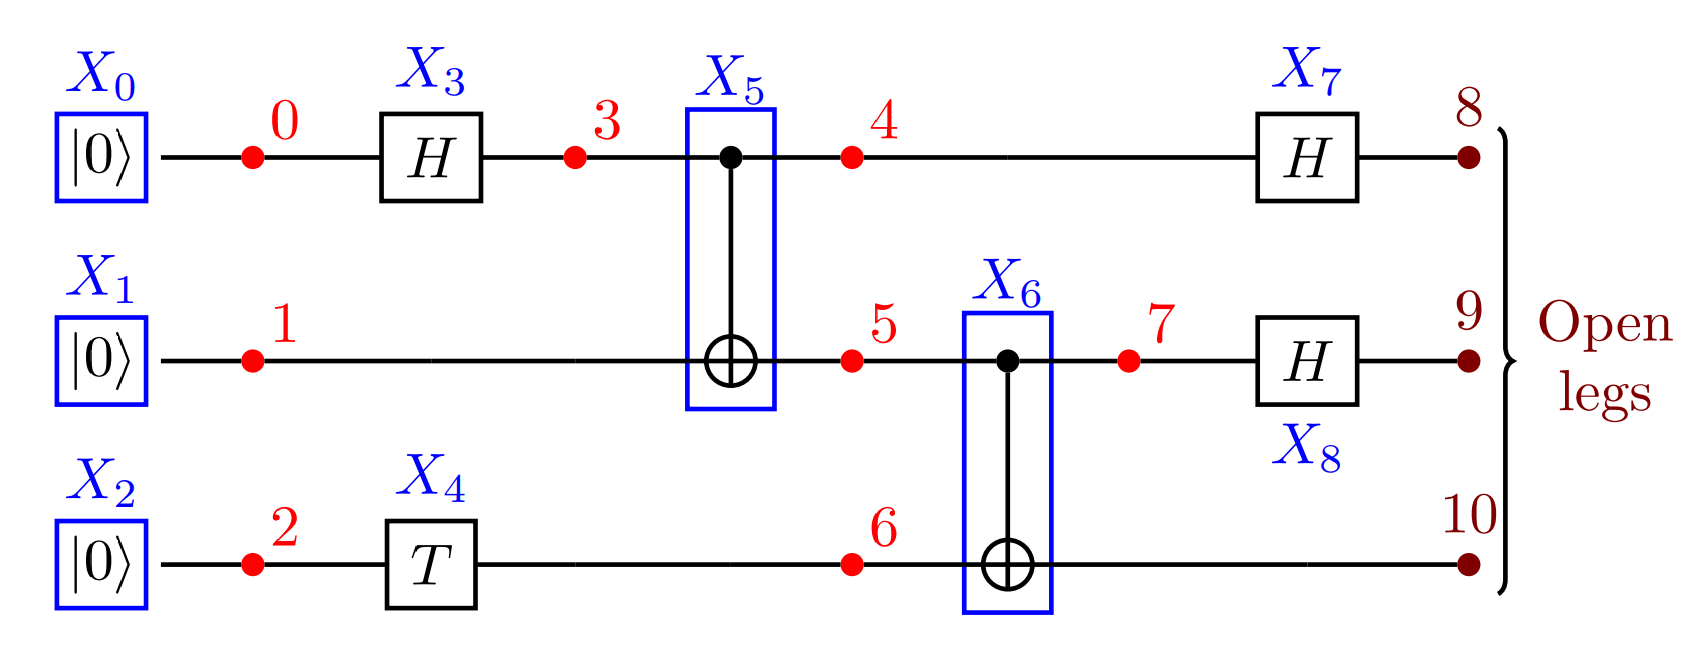
\includegraphics[width=\textwidth]{images/6_3_circ.png}
        \caption{量子线路。}
        \label{6_3_circ}
    \end{subfigure}
    \begin{subfigure}{0.4\textwidth}
        \centering
        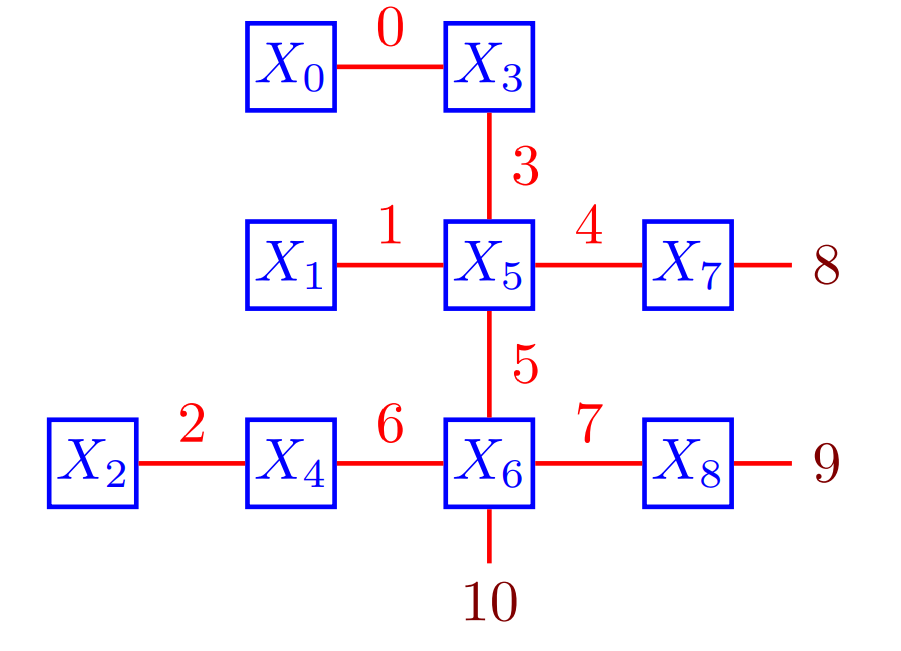
\includegraphics[width=0.9\textwidth]{images/6_3_tn.png}
        \caption{张量网络。}
        \label{6_3_tn}
    \end{subfigure}
    \caption{量子线路及其对应张量网络示例。}
    \label{fig:6_3_tn_circ}
\end{figure}

以图 \ref{fig:6_3_tn_circ} 为例，$(X_{0}, \ldots, X_{8})$ 是该张量网络中的张量。我们用数字 0--7 表示张量腿，并用数字 8--10 表示开放腿。

直接应用张量方法通常会随着量子比特数和线路深度增加而导致复杂度呈指数增长，使得大规模线路难以在合理时间内完成模拟。然而，如果模拟只计算线路末端的一个或一小批状态振幅，那么张量网络的复杂度将受收缩过程中最大张量的大小限制。该大小又随张量网络对应图的树宽呈指数增长 \cite{Markov_2008}。

在 \QuPack\ 中，我们提供了一种用于计算单振幅和多振幅的超高速张量网络模拟方法 \cite{kalachev2022multitensor}，同时也提供了面向数百量子比特的线路采样模拟能力。此外，我们还在张量网络模拟中实现了量子噪声信道，从而能够模拟超大规模真实量子芯片的行为。
% \begin{figure}[h]
%   \begin{center}
%     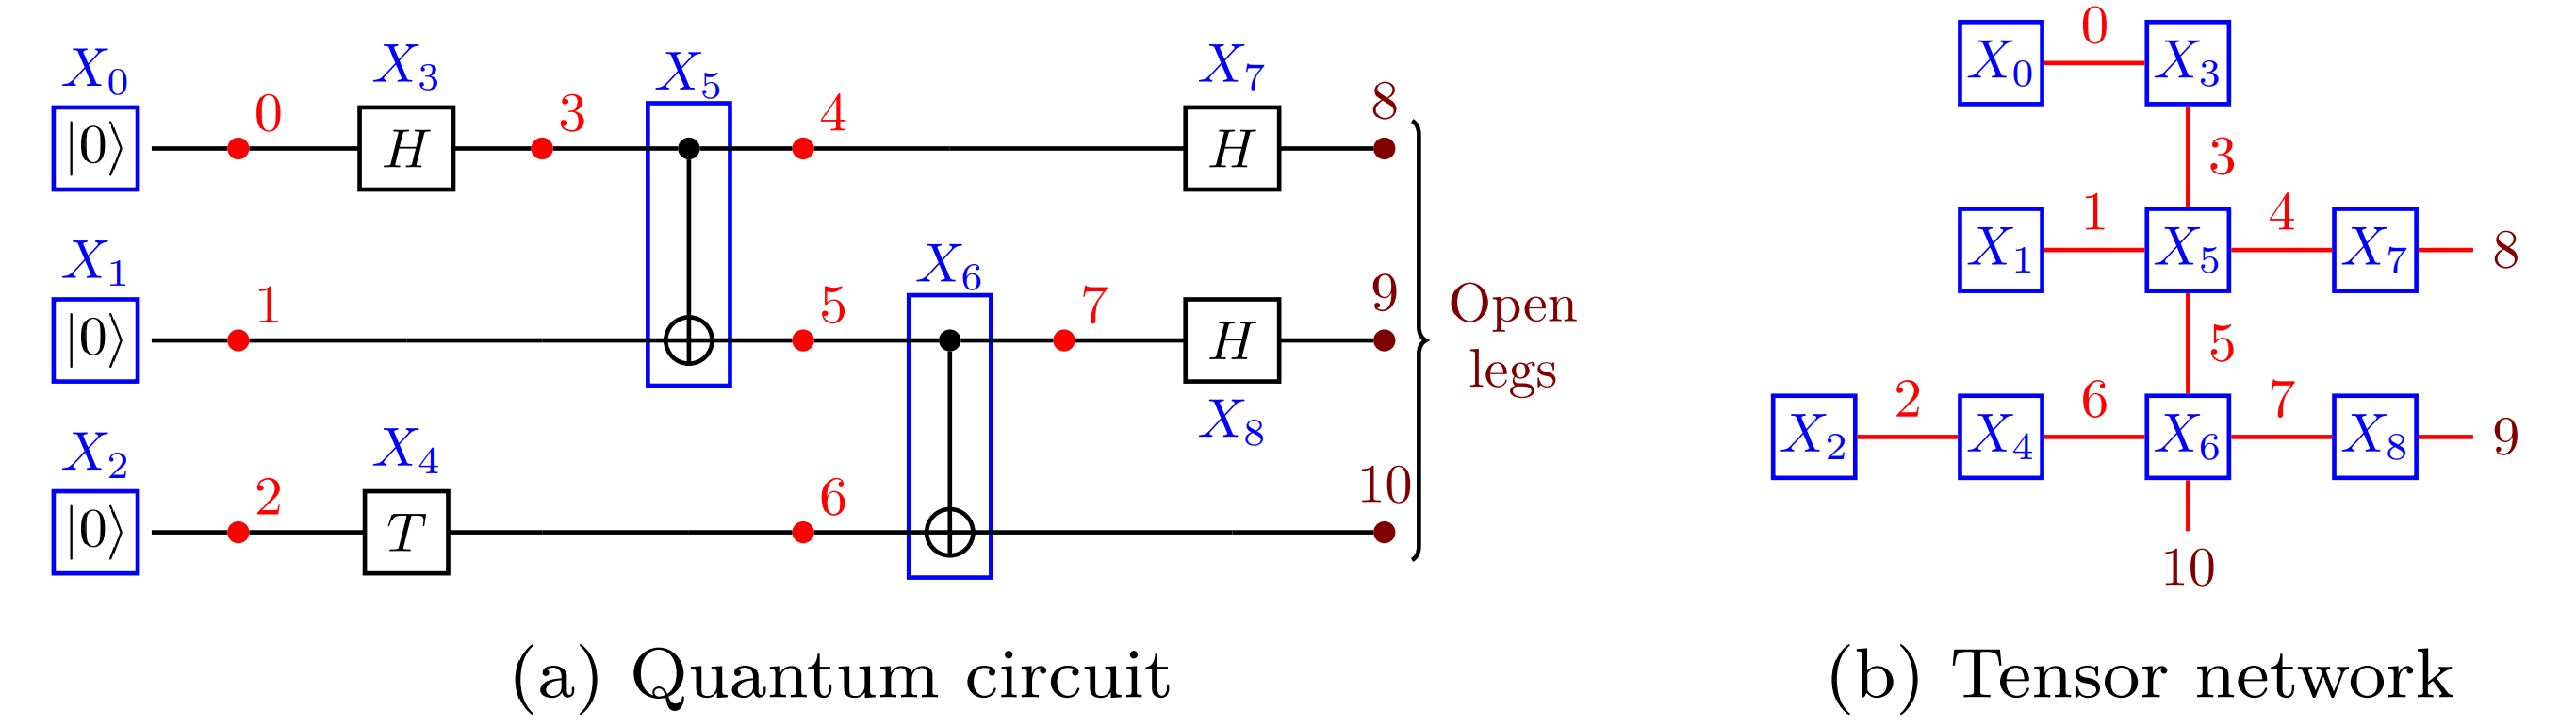
\includegraphics[width=0.9\linewidth]{images/6_3_tn_circ.png}
%   \end{center}
%   \caption{Example for quantum circuit and tensor network.}
%   \label{fig:6_3_tn_circ}
% \end{figure}

\subsubsection{基本用法}
下面将详细说明该张量网络模拟器的使用方法。
该模块支持以下功能：采样、期望值计算和振幅计算。

\textit{采样与期望值} -- 其用法与 \MindQuantum\ 中的方法完全相同。实际上，我们只是将张量模拟器 \code{MQ_TNSim} 封装为 \MindQuantum\ 模拟器的一个后端，因此它仍然支持原有的所有功能。
\begin{lstlisting}
from qupack.tensor import MQ_TNSim
sim = Simulator(MQ_TNSim(n_qubits=n_qubits), n_qubits)
res = sim.sampling(circ, shots=shots)
\end{lstlisting}

\textit{振幅计算} -- 振幅计算是张量网络模拟器中的一项特定功能。尽管全振幅计算本身已经包含所有振幅，因此不需要单独提供这一功能，但振幅计算在某些过程中起着关键作用，例如 XEB 计算和大规模线路采样任务。因此，在这一场景中，张量网络模拟器 \code{TNSimulator} 专门用于振幅计算。

\begin{lstlisting}
from qupack.tensor import TNSimulator
sim = TNSimulator(circuit_file='data/circuits/simple/circuit_n12_m14_s0_e0_pEFGH.qsim', backend='numpy')  # available backends : numpy, cupy, csim
n = sim.qubit_count
bitstring = [randint(0,1) for i in range(n)]
amp = sim.get_amplitude(bitstring)
\end{lstlisting}

初始化 \code{TNSimulator} 时，可以针对不同任务指定以下后端：
\begin{itemize}
    \item numpy --- CPU 上用于张量操作的标准库。对于简单线路速度最快，但在多振幅模拟模式下非常慢。
    \item cupy --- GPU 张量收缩后端。适用于中等复杂度线路。
    \item csim --- 模拟器的 CUDA 实现。对于较长模拟（> 10 秒）速度最快，但在较简单情形下存在较明显额外开销。
\end{itemize}

除了单振幅计算之外，它还支持多振幅和批量振幅计算：
\begin{lstlisting}
# batch-amplitudes
amps = sim.get_batch(bitstring, output_idx=[0,1,2])
# multi-amplitudes
amps = sim.get_amplitudes(bitstrings)
\end{lstlisting}
